% Copyright 2009 Wilfred Hughes, CC-BY license
\documentclass[12pt,twoside,notitlepage]{report}

\usepackage{a4}
\usepackage{verbatim}

% for pretty printing grammar in BNF
\usepackage{bnf}
\usepackage{color}

\usepackage{graphicx}

\input{epsf}                            % to allow postscript inclusions
% On thor and CUS read top of file:
%     /opt/TeX/lib/texmf/tex/dvips/epsf.sty
% On CL machines read:
%     /usr/lib/tex/macros/dvips/epsf.tex

\raggedbottom                           % try to avoid widows and orphans
\sloppy
\clubpenalty1000%
\widowpenalty1000%

\addtolength{\oddsidemargin}{6mm}       % adjust margins
\addtolength{\evensidemargin}{-8mm}

\renewcommand{\baselinestretch}{1.1}    % adjust line spacing to make
                                        % more readable
\begin{document}

\bibliographystyle{plain}


%%%%%%%%%%%%%%%%%%%%%%%%%%%%%%%%%%%%%%%%%%%%%%%%%%%%%%%%%%%%%%%%%%%%%%%%
% Cover sheet


\pagestyle{empty}

\hfill{\LARGE \bf Wilfred Hughes}

\vspace*{60mm}
\begin{center}
\Huge
{\bf oosh: An object oriented shell} \\
\vspace*{5mm}
Computer Science Part II \\
\vspace*{5mm}
Churchill College \\
\vspace*{5mm}
\today  % today's date
\end{center}

\cleardoublepage

%%%%%%%%%%%%%%%%%%%%%%%%%%%%%%%%%%%%%%%%%%%%%%%%%%%%%%%%%%%%%%%%%%%%%%%%%%%%%%
% Proforma, table of contents and list of figures

\setcounter{page}{1}
\pagenumbering{roman}
\pagestyle{plain}

\chapter*{Proforma}

% fixme: wordcount at completion
{\large
\begin{tabular}{ll}
Name:               & \bf Wilfred Hughes                       \\
College:            & \bf Churchill College                     \\
Project Title:      & \bf oosh: An object oriented shell \\
Examination:        & \bf Computer Science Part II, 2009-2010        \\
Word Count:         & \bf 1587 \\
Project Originator: & \bf Wilfred Hughes                    \\
Supervisor:         & \bf David Eyers                    \\ 
\end{tabular}
}

\section*{Original Aims of the Project}

I planned to write a Unix shell from scratch in Python. It
would enforce a data structure on data piped between processes, so
programs can reason about data at a higher level. It would also enable
transparent network access using a lazy data fetch. Finally, the shell
syntax would be simplified to minimise command length for common
instructions.

\section*{Work Completed}
% fixme: less than 100 words, but proforma cannot exceed one page
I created an interactive shell with support for both new data-aware commands and
traditional Unix commands. It also offers a basic command history and pretty
prints all structured data.

I created a set of commands which understand the data structure I defined. These
included commands which produce data, commands that manipulate data and an
automatic graphing utility.

% fixme: repeats 'lazy' terminology from above
For networking I created a server that permits users to log in and execute
commands as if they were being run locally. The client then fetches data lazily
from the server.

\section*{Special Difficulties}
None.
 
\newpage
\section*{Declaration}

I, Wilfred Hughes of Churchill College, being a candidate for Part II
of the Computer Science Tripos, hereby declare that this dissertation
and the work described in it are my own work, unaided except as may be
specified below, and that the dissertation does not contain material
that has already been used to any substantial extent for a comparable
purpose.

\bigskip
\leftline{Signed}

\medskip
\leftline{Date}

\cleardoublepage

\tableofcontents

\listoffigures

\newpage
\section*{Acknowledgements}

There have been three previous part II projects in this area that I am
aware of. I have examined them briefly, but they explored different
shell topics to Oosh. These are J.\ Tippell in 2006, J.\ Harbin in
2005 and G.\ Beasley in 2003.

%%%%%%%%%%%%%%%%%%%%%%%%%%%%%%%%%%%%%%%%%%%%%%%%%%%%%%%%%%%%%%%%%%%%%%%
% now for the chapters

\cleardoublepage        % just to make sure before the page numbering
                        % is changed

\setcounter{page}{1}
\pagenumbering{arabic}
\pagestyle{headings}

\chapter{Introduction}

\section{Historical Motivations}
The command line shell (henceforth \emph{shell}) is one of the earliest user
interfaces in the history of computing, with recognisable shells having appeared
by 1965 \cite{multics} on the Multics system. A shell offers the user a
convenient abstraction to interact with his system. He may perform common tasks
using considerably shorter commands than using his programming language of
choice. A shell scripting language, therefore, has always been an exchange of
power for brevity.

The earliest shell that included modern shell features was the Bourne
shell (known as {\tt sh}), developed by Stephen Bourne. It was
released in 1977 as a part of Version 7 Unix. The most common shell in
use today is Bash, which offers a superset of the features of {\tt
  sh}. Bash seeks backwards compatibility with the Bourne shell
wherever possible. Sadly the Bourne shell was a result of hacking and
experimentation, so later attempts to retroactively produce a formal
grammar that describes its behaviour have failed \cite{bourne}.

This pursuit of backwards compatibility has resulted in today's shells
being optimised for common use cases that are outdated. The language
syntax they accept is unnecessarily complex, making it hard for the
user to exercise confidence in writing scripts. Further the language
has not been expanded or changed to make tasks that are typical today easier.

I revisited these assumptions. How could I make today's common shell
usage simpler? What other use cases would be desirable but are not
supported by shells that are currently available?

\section{The Purpose Of The Shell}
I wanted to reconsider what it meant to be a shell. A shell is not as
expressive as a programming language. Shell scripting languages have
far fewer primitive data structures. They only offer a very limited
range of arithmetic operations, usually only basic integer maths.

Today's scripting languages fill a different niche. Python and Ruby
have both become popular and both offer an interactive mode of
operation. However they are more general purpose and so their syntax
is too heavyweight for the typical system administration tasks that
shells are used for. A simple directory listing in Python requires the
user to {\tt import os} to import the necessary libraries then to run
{\tt for x in os.listdir('.'): print(x)}. A shell is set up for
precisely this type of task.

A shell therefore has many implicit assumptions. Almost everything is
expected to be handled by an external process according to the Unix
design philosophy of ``do one thing and do it well''. As a result
arithmetic is handled by {\tt bc}, file deletion by {\tt rm},
compression by {\tt gzip}, and so on. As a result administration tasks
become much easier in a shell than using a full scripting language
interpreter.

\section{Existing Solutions}
% feature matrix/table?
I evaluated several well-known shells available today. One of the most popular
options is Bash, which is the default on GNU/Linux and Mac OS X.

A more recent alternative to Bash is the Friendly Interactive Shell (`Fish'),
released in 2005. Fish is not a substantial departure from Bash, but breaks
backwards compatibility. The design of Fish \cite{fishdesign} is motivated by a
desire to create a minimal, orthogonal scripting language. While it achieves
these goals it still requires the user to perform dumb manipulations on
unstructured text.

Another recent development is PowerShell, a Microsoft scripting language and
shell released in 2006. PowerShell is a more radical departure from traditional
shell design, offering an object-oriented approach. Whilst this offers an
increase in expressive power, the PowerShell design does not seek to optimise
the interface for interactive usage. PowerShell cmdlets use a more verbose
noun-verb naming scheme and the programmer is sometimes exposed to underlying
Windows API for simple tasks such as basic networking.

None of these existing solutions have support for transparent
networking. Bash-like shells require the user to {\tt ssh} into the
desired system, so building a pipeline with commands on varying hosts
is non-trivial. PowerShell solutions are more heavyweight and vary for
the cmdlet used. Some Powershell cmdlets take a host as an argument
whereas others take a network session object argument.

\section{My Design}

As a result I decided to create a completely new shell with a new
language that would be similar to experienced shell. I would
re-evaluate design decisions made by previous shell developers. My
design would seek to make today's common shell tasks easier.

In addition to the language I would develop a data format that enable
command line tools to output data in a more structured manner and
include metadata that was machine-readable. To demonstrate the
versatility of this data structure I would create a number of programs
that could produce and/or manipulate data in this format.

Since networking is much more prominent part of today's computer usage
I concluded that my shell should include networking as a built-in
rather than leaving it to an external program. This would require me
to develop a simple client/server architecture. Since the shell itself
would be aware of where commands were running, it would be able to use
a intelligent data transfer scheme to minimise bandwidth.

\cleardoublepage

\chapter{Preparation}

\section{Requirements}
I needed to create a shell that would be familiar to an experienced shell user,
so my shell should follow shell conventions where sensible. Any shell that hopes
to be be useful for a majority of users must be compatible with existing Unix
commands as there are simply too many to reimplement all of them for a new
design. My shell therefore needed to support the commands already available on
the user's system.

The scripting language that my shell would accept needed to be
familiar to users of common shells available today. Any changes made
needed to be justified as to how they made common use cases
simpler. This included examining the pipeline metaphor in some depth
and expanding upon it. One common use case is developing a shell
command incrementally, whilst only being interested in the output of
the final command. I concluded that the shell required the ability to
save intermediate pipelines in a lightweight fashion.

I also needed to develop a data structure that would enable my
programs to process data at a higher level. With my desire to work
with current programs and aiming to maintain useful shell metaphors, I
needed to preserve the basic concept of a pipeline as far as
possible. This meant local commands needed to use the POSIX pipe
primitive when pipelines were local. Since I wished to support
interleaving of my commands and other commands, I required a data
structure that was transmitted as structured text.

With my data structure in place I needed a set of commands that would
demonstrate the versatility of my design. This set needed to include commands
that would produce structured data, commands that could manipulate this data and
commands that would offer visualisations of this data.

%todo: expand me
Finally, I wanted my shell to support a convenient network abstraction. This
required a simple client/server architecture and a lightweight syntax to
support it.

\section{Development Approach}
Since my design aimed to build on traditional shell design, extending
an existing shell was an option worth considering, particularly since
most Unix shells are available under an open-source license. I
investigated building on top of Bash or Fish, but both of these were
substantial pieces of C code, most of which would require major
changes to work with my intended features. For example, Fish uses a
custom parser which is approximately 2000 lines of C code. Compatibility
with existing shells did not offer any obvious benefits for the
additional effort. I concluded that starting afresh was my best
option.

Since I was developing a tools for a modern Unix system, I chose a workflow that
followed today's Unix coding practices. I chose to write my shell in Python, a
modern scripting language, used Emacs as my editor and used Git, a distributed
version control system to track changes. By the same logic I chose to host my
code on GitHub, which had the additional benefit of acting as an off-site
backup. Later on I needed a parser and lexer so chose Python implementations of
Lex and Yacc as these are also standard tools.

My initial specification was very broad, which enabled me to use a
fairly exploratory style of coding. My final grammar is in figure
\ref{grammar} and was developed iteratively after researching the
syntax used in Bash and Fish. This grammar was created to provide a
useful subset of Fish functionality and be syntactically similar.

Ultimately a mainstream shell is a very large body of code (for
example, Bash 4.1 contains over 140,000 lines of C
code\footnotemark[1]) and so I could not hope to replicate all this
functionality in the time available. My objective then became to
produce a proof-of-concept shell that demonstrated the advantages of
my design.

\footnotetext[1]{Calculated by running {\tt find . -name '*.[ch]' | xargs wc -l}
  on the source code of Bash 4.1.}
\stepcounter{footnote}

% bash and Fish: no proper grammar. hard to change guts for more radical
% features, no hackable grammar
% python offered cmd.py which is skeleton shell
% networking easier in python, text manipulation particularly so

%% Typical CLI commands are developed iteratively, which is why commands print
%% their usage guidelines if used incorrectly. Pipeline saving allows the user to
%% develop his pipelines more incrementally.

% investigation -- compared to existing systems
%   -- bash, Fish, powershell, osh (Timoth Budd 1989), REPLs, cmd.exe
%     -- macro language vs programming language
%   -- bash particularly: lex and parse approach, backwards compat
% requirements (from proposal)
% development approach -- development environment, VCS, backup
%   -- system design -- diagrams of structure!
%   -- different implementation approaches considered
%     -- modify existing work, start from scratch
%     -- similar grammar, readily piped to system below?
% theory?
% summary

% quote: The grammar presented in Bourne's paper describing the shell
% distributed with the Seventh Edition of Unix is so far off that it does not
% allow the command who|wc. In fact, as Tom Duff states:

% The POSIX.2 standard includes a yacc grammar that comes close to capturing the
% Bourne shell's behavior, but it disallows some constructs which sh accepts
% without complaint-and there are scripts out there that use them.

\cleardoublepage

\chapter{Implementation}
% features:
% strict data format
% interleave new commands
% primitive namespacing
% familiar syntax

The final result of my project was the shell client itself, a simple server and
a selection of commands that understood the oosh data structures. I also wrote
some simple scripts to demonstrate the power and flexibility of my design.

(diagram of file layout)

In each section I give an example of this feature being used, along
with its resulting output. This should clarify how these techniques
work in practice.

\section{Pipelines}
A major focus of Oosh's design is making the concept of pipes more powerful than
the options available on competing shells. Oosh generalises the concept of pipes
to enable multiple commands to have their output piped into a single input. It
also permits convenient pipe saving for later access. Pipes also work over a
network transparently to the user.

\subsection{Pipe Saving}
A common way of using today's shells is to iteratively write
instructions. Many Unix commands recognise this approach and so print
a simple help message if called without any arguments. Oosh commands
also follow this convention. A system
administrator, trying to fix a KDE application, may build up a Bash
command as shown in figure \ref{bashiter}.

\begin{figure}[h]
\label{bashiter}
\caption{Iterative shell usage with Bash}
\begin{verbatim}
$ ls /usr/lib
$ diff /backup/20100120/usr/lib /usr/lib
$ diff /backup/20100120/usr/lib /usr/lib | grep libkde
\end{verbatim}
\end{figure}

In this example he is repeatedly reading {\tt /usr/lib}. Each command rereads from
this folder unnecessarily. As the command gets longer he is no longer interested in
the earlier processes. The Oosh solution here is to allow him to save this data so
that he can access it again later, whilst only worrying about the current filter
operations he is performing. This is shown in figure \ref{ooshiter}.

\begin{figure}
\label{ooshiter}
\caption{Iterative shell usage with Oosh}
\begin{verbatim}
$ oosh_ls /usr/lib |1
$ oosh_ls /backup/20100120/usr/lib |2
$ |1+2 oosh_difference |3
$ |3 grep libkde
\end{verbatim}
\end{figure}

The administrator is now able to reason about previously generated data in a
simpler manner. He can also refer back to previously generated results
even if he cannot generate the data again.

An experienced Bash user could use output redirection to achieve the
same effect as the Oosh example. This is discussed in section
\ref{commandlength}. However the Bash redirection syntax is less
concise, so the equivalent commands are not as short or as readable.

For pipeline saving I reused the pipe character to clarify that pipe
saving is similar to the pipeline metaphor and can be used in a
similar way.

\subsection{Multipipes}

The traditional pipeline metaphor only allows one pipe into a
program. A Bash user is forced to write each output out to a file
somewhere if he wishes to use commands such as {\tt cat} or {\tt
  diff}.

The Oosh approach is rather different. Oosh enables programmers to
write programs that take two inputs in order to do more powerful
computations. Initially I considered allowing an arbitrary number of
inputs but the additional complexity offered no clear benefits so I
limited my design to only one or two input commands.

Since I modelled my data manipulation on the relational algebra, I
implemented {\tt oosh\_union}, {\tt oosh\_difference} and {\tt
  oosh\_product} based on their corresponding operators. This
`multipipe' design seemed natural for these operators. To demonstrate
that this was a generalisation of a pipe I chose a syntax that was
very similar to the pipe saving syntax.

\begin{figure}
\caption{An example of sequential commands, pipeline saving and multipipes}
\begin{verbatim}
4$ oosh_ps |1; sleep 1m; oosh_ps |2; |1+2 oosh_difference
Command CPU % Memory % PID  User
python3 0.0   0.3      6081 wilfred
sh      0.0   0.0      6082 wilfred
ps      0.0   0.0      6083 wilfred
\end{verbatim}
\end{figure}

\subsection{Pipes over networks}

A design principle used in Oosh was to examine how computer usage has
changed and how today's shells could work better in these different
use cases. It quickly became clear that networking is cumbersome and
it would be better if pipes worked over networks as if they were
local.

A Bash user has two options when working with remote systems: he can
either mount the remote system on his local system, or use {\tt
  ssh}. If he mounts the remote system all computation must be
performed on his local system. If he {\tt ssh} he must either start a
shell session remotely and create files to {\tt scp} (copy over {\tt
  ssh}) back or use {\tt ssh} for each command individually.

The Oosh solution is easier to work with. The user must {\tt connect}
to each of the remote systems he wishes to work with, then any
commands may be run on any system at the users discretion without
further authentication. For this I chose the simplest syntax I could,
requiring the user to only write {\tt mycommand@myserver} to instruct
Oosh to run a command on a specific system. As discussed in section
\ref{networking}, if the user does not specify then Oosh attempts to
minimise bandwidth consumption. This syntax is modelled on that of
email, which should make Oosh scripts readable to new users.

\section{Data Structures}
My initial design was to have structured data pass through pipes between the
commands, but this still left me with a variety of implementation
possibilities. The data I wanted to manipulate turned out to fit a tabular
format well, so as I iteratively developed the data structure I
focused on a representations where the data was separated into rows
with metadata.

 focused on a representation of each line of data
with labels. %unclear, clarify

One of the initial ideas was to use an object oriented programming
approach, so my first prototype used an object which encapsulated
a row. However successive refactorings reduced this object to the point
I was able to replace it entirely with Python {\tt dict}s (the mapping
structure primitive in Python).

Another design criterion was the data structure had to be passed as
text between processes if I wanted to use underlying Unix
inter-process communication. This again pushed me towards using
standard Python primitives so that I was able to write out a text
representation using {\tt \_\_repr\_\_()} and convert it back using
{\tt eval()} without having to write any conversion code myself.

My final design separates lines of structured data with the newline
character in the text stream. This enables the interleaving of
existing line-oriented Unix commands and Oosh commands whilst still
preserving the data format. The examples in sections \ref{lsexample}
and \ref{forexample} demonstrate this. Since all the metadata is
stored within each line, there is no risk of commands like {\tt tail}
removing the header of the data as there is with Bash.

\subsection{Pretty Printing}
\label{prettyimpl}
Since traditional Unix commands output data in an unstructured way, output forms
vary widely. In contrast, Oosh enforces its format, so it naturally follows to
spend more development time on an attractive pretty print that is run by the
shell on all conformant data.

The pretty print functionality I developed is coloured, uses character-perfect
layout and supports heterogeneous lines of data. This ensures that each column
is printed at optimum width dependent on the length of the entries.

The algorithm I designed takes lines of Oosh output as input and finds
the optimum layout. This is $O(C \log C + CL)$ time, where $L$ is the
number of lines, and $C$ the number of columns. I benchmark this
later. %todo: add section number

The disadvantage of my design is that it requires that a command
entered by the user must have finished being evaluated before the
output can be pretty-printed and shown to the user. However, it is
only really necessary that one screenful of data is printed in a
character perfect manner, so if the Oosh shell was rewritten with
curses (curses is a library used for creating full screen interfaces
for text tools) based interface then this problem would be
alleviated. Furthermore, a data set which looked like:

\begin{verbatim}
{'Name': 'Jim', 'Age': 10}
{'Name': 'John', 'Age': 36}
...
{'Name': 'Slartibartfast the Magrathean', 'Age': 68}
\end{verbatim}

would always print the name column very wide in Oosh, even if the last
line is not visible on screen. A curses-interface would work better in
this case as it would find the optimum display for that screenful
rather than the global optimum.

% but by benchmark, even 50k producing data is acceptable

% nice example would be to show that tail does not remove the table header

\subsection{Data Example}
\subsubsection{Raw Data}
\label{rawdata}
% fixme: fix incorrect quoting in output
\begin{verbatim}
{'Owner': 'wilfred', 'Size': 1013234, 'Filename': 'uucp-1.07.tar.gz'}
{'Owner': 'wilfred', 'Size': 1152997, 'Filename': 'fish-1.23.1.tar.gz'}
{'Owner': 'wilfred', 'Size': 1837, 'Filename': 'smlnj.tar.gz'}
{'Owner': 'wilfred', 'Size': 6598300, 'Filename': 'bash-4.1.tar.gz'}
{'Owner': 'wilfred', 'Size': 196529, 'Filename': 'xwrits-2.26.tar.gz'}
{'Filename': 'plasma-weather-0.4.tar.gz', 'Size': 2480099}
\end{verbatim}
Note we have rudimentary types here, distinguishing between strings and
integers. The sort commands in Oosh take advantage of this.

\subsubsection{Pretty Print Output}
% fixme: need to emulate shell colouring
% fixme: discuss character perfect print, unifying disparate data, relation to
% pipe saving
\begin{verbatim}
Filename                         Owner   Size      
uucp-1.07.tar.gz                 wilfred 1013234   
fish-1.23.1.tar.gz               wilfred 1152997   
smlnj.tar.gz                     wilfred 1837      
bash-4.1.tar.gz                  wilfred 6598300   
xwrits-2.26.tar.gz               wilfred 196529    
plasma-weather-0.4.tar.gz        -       2480099
\end{verbatim}

\section{Syntax}
When I developed the first parts of Oosh I did not specify a grammar and simply
modified the syntax that the prototype accepted as I went along. When I
implemented a full interpreter I formalised the syntax I had developed. This
approach enabled me to experiment without having to radically restructure the
code at each iteration.

Oosh supports normal conditionals based on process return codes, two
different types of loops, string variables, pipe variables (which I
refer to as `saved pipes') and command pipelines. This is a smaller
feature set compared with more mature offerings such as Bash and
Fish. However it is sufficient for basic shell interaction, and the
parsing and evaluation code has been written in a sufficiently
flexible manner that any desired expansion could be added with minimal
difficulty.

The design for variables deserves closer attention. The Oosh design
can be seen as two variable namespaces, one that holds strings and the
other that saves the output of pipes. Saved pipes may be emulated in
bash by executing {\tt command1 >/tmp/foo} and then later {\tt command2
  </tmp/foo}. However this approach requires the user to explicitly
create temporary files and does not conveniently generalise to network
access, which requires {\tt scp} as well. Saved pipes are therefore
only a convenience for the user, not a completely novel use case.

Other notable omissions from this design include subshells (backticks
in Bash usage), arithmetic operations, function definitions, array
variables and non-interactive usage. This turns out to rarely be a
problem for the user. Subshells can be emulated with pipe
saving. Arithmetic operations may be performed using the Unix {\tt bc}
command, which is arguably a more Unix style design (conforming to the
``do one thing and do it well '' design mantra). The remaining
omissions are more difficult to work around but fall outside of the
use cases being explored in Oosh.

\begin{figure}[h]
\label{grammar}
\caption{A formal specification of the language accepted by Oosh}
\begin{grammar}
      [(colon){$::=$}]
      [(semicolon){$|\,$}]
      [(nonterminal){$\langle$}{$\rangle$}]
      [(quote){}{}] % grim hack since ; has meaning so we use ";"
<commands> : <commands>";" <commands>\\
% grim hack to force indentation
\textcolor{white}{tab};commands NAMEDPIPE\\
\textcolor{white}{tab};<while> ;<if> ;<assign> ;<for> ;<command> ;$\epsilon$

<for> : for STRING in <values>";" do <commands>";" end

<while> : while <command>";" do <commands>";" end

<if> : if <command>";" do <commands>";" end\\
\textcolor{white}{tab};if <command>";" do <commands>";" else do <commands>";" end

<assign> : set STRING <value>

<command> : <simplecommand>\\
\textcolor{white}{tab};NAMEDPIPE <simplecommand>\\
\textcolor{white}{tab};MULTIPIPE <multicommand> PIPE <simplecommand>\\
\textcolor{white}{tab};MULTIPIPE <multicommand>

<values> : <value> <values> ;<value>

<value> : STRING ;VARIABLE ;QUOTEDSTRING

<simplecommand> : <values>
;PIPE <simplecommand>
    
<multicommand> : <values>
\end{grammar}
\end{figure}

\subsection{Simple Pipelines}

I performed an examination of an online command-line snippets
repository \cite{clifu} and the official Bash reference manual
\cite{bashman}. I concluded that the pipeline is the most frequently
used and earliest taught shell command. The Oosh pipeline syntax is
immediately familiar to a shell user, without any different syntax
required for structured data or unstructured data. It is so similar
that many simple shell invocations will work unchanged in Oosh. Figure
\ref{lsexample} gives an example of this feature in use.

\begin{figure}
\label{lsexample}
\caption{A simple pipeline showing contextual data manipulation. Note tail is a part of
GNU coreutils and is working in Oosh without modification.}
\begin{verbatim}
1$ oosh_ls /usr/bin | oosh_project Filename Size | oosh_sort Size | tail
Filename Size
mencoder 10984340
inkview  11074508
inkscape 11100236
mplayer  11758932
bibtexu  17312116
xetex    17799216
xelatex  17799216
skype    18567888
\end{verbatim}
\end{figure}

\subsection{Control Structures}
\label{forexample}

Control structures vary quite widely between shell offerings. One
perceived weakness of Bash is that blocks are closed using different
keyword depending on the control structure used. For example, a {\tt
  for} loop syntax ends with {\tt end}, an {\tt if} block ends with
{\tt fi} and a function declaration ends with {\tt \}}. Fish fixes
this weakness (at the expense of POSIX compliance) by always using
{\tt end}. I felt that this made writing shell scripts easier so the
Oosh syntax is very similar to Fish here.

Figure \ref{forloop} shows the user using a {\tt for} loop.

\begin{figure}
\label{forloop}
\caption{An example {\tt for} loop in Oosh, demonstrating variable
  assignment and unstructured data}
\begin{verbatim}
3$ for x in 131.111.8.42 131.111.12.20 131.111.131.1; do ping $x -c 1; end
PING 131.111.8.42 (131.111.8.42) 56(84) bytes of data.
64 bytes from 131.111.8.42: icmp_seq=1 ttl=252 time=0.400 ms

--- 131.111.8.42 ping statistics ---
1 packets transmitted, 1 received, 0% packet loss, time 0ms
rtt min/avg/max/mdev = 0.400/0.400/0.400/0.000 ms
PING 131.111.12.20 (131.111.12.20) 56(84) bytes of data.
64 bytes from 131.111.12.20: icmp_seq=1 ttl=252 time=0.433 ms

--- 131.111.12.20 ping statistics ---
1 packets transmitted, 1 received, 0% packet loss, time 0ms
rtt min/avg/max/mdev = 0.433/0.433/0.433/0.000 ms
PING 131.111.131.1 (131.111.131.1) 56(84) bytes of data.
64 bytes from 131.111.131.1: icmp_seq=1 ttl=63 time=0.338 ms

--- 131.111.131.1 ping statistics ---
1 packets transmitted, 1 received, 0% packet loss, time 0ms
rtt min/avg/max/mdev = 0.338/0.338/0.338/0.000 ms
\end{verbatim}
\end{figure}

\section{The Shell}
The Oosh client is the largest single piece of code and can function without a
server. Basic command line interaction is provided by the {\tt cmd.Cmd} object
in the standard Python library. This meant the shell had supported basic user
interaction and command history from very early on, allowing me to test the
system as a whole. I was then able to add functionality and complexity
iteratively, with the code largely functional at any given point in time.

The shell itself takes input from the user on a line-by-line basis. Each line is
lexed, parsed and the resulting parse tree is evaluated.

% (simplified) picture of parse tree needed
Within each pipeline % have pipelines been explained by this point?
a {\tt PipePointer} is passed along to abstract away the actual location of the
data. This enables the shell to use Unix pipes locally % would be good to benchmark this
but still move data across the network as needed.

\section{Networking}
\label{networking}
% need intro para

The networking functionality was designed with two intentions: a concise,
convenient syntax and efficient bandwidth usage. Today a user can use Bash and
SSH to run commands remotely, but running successive commands on different
systems is not convenient.

\begin{figure}
\caption{Collecting data remotely and performing analysis locally
  using Bash}
\begin{verbatim}
home$ ssh wilfred@remote.com
remote$ ps > /tmp/ps.txt
remote$ exit
Connection to remote.com closed.
home$ scp wilfred@remote.com:/tmp/ps.txt .
home$ grep root <ps.txt 
\end{verbatim}
\end{figure}

\begin{figure}
\caption{Collecting data remotely and performing analysis locally
  using Oosh}
\begin{verbatim}
$ connect@remote.com wilfred password
$ ps@remote.com | grep@localhost root
\end{verbatim}
\end{figure}

I firstly extended the Oosh syntax to allow this simple location
specification using a hook in the evaluator (hence this is not shown
in the grammar specification). I then required a server/client
architecture that would enable the user to run remote commands from
his Oosh client as if they were local.

The server is a very simple design, only permitting one user to interact at any
one point. Using the client, the user specifies the location where he wishes
commands to be run. Once the user has logged in to a remote server, the client
will automatically initiate commands on the server. Since the client collects
data on the users behalf we can send the data lazily.

The server supports the following commands: {\tt connect}, to
authenticate a new user, {\tt
  disconnect}, to deauthenticate, {\tt send}, to send the results of
the last command back to the client, {\tt receive}, to send data to
the server for it to use as {\tt stdin} to the next command, and {\tt
  command}, to execute a shell command on the server. 

The client initiates a connection on the Oosh port, 12345, then
authenticates and begins sending {\tt command} strings for the server
to execute. The server runs these commands with the privileges of the
user who started the server. A mature implementation would need to do
a thorough security audit, particularly since there is no protection
between different users logged in at the same time. 

Each command sent to the server corresponds to a simplecommand in the
grammar, so if the user enters the command {\tt a@remote | b@remote |
  c@remote} this will become three separate messages to the server,
{\tt command a}, {\tt command b}, {\tt command c} with the pipe being
implicit. Therefore a loop where every simplecommand in the body is
specified to be run remotely will result in every simplecommand
producing a {\tt command} message to be sent to the server. This is
not a performance problem under the assumption that the amount of data
sent between processes vastly exceeds the number of simplecommands
that need sending.

Since the Oosh server only sends the results of computation back on
demand, it enabled me to use a lazy data approach. Again if we
consider {\tt a@remote | b@remote | c@remote}, only the result of the
computation after {\tt c} has terminated will be sent back to the
client. This optimisation is transparent to the user and does not
affect results.

A more interesting optimisation in Oosh is that of `command moving'. If
the user runs the command {\tt oosh\_ps@remote | oosh\_project Command
  PID} the {\tt oosh\_project} command acts as a filter and is
location independent. Oosh recognises these commands (using a simple
whitelist) and runs them on the same system as the previous command to
reduce bandwidth consumption. This is safe (it does not change
results) and is transparent to the user. The user may however
explicitly state where a command is to be run and Oosh will respect
that. The actual logic to decide to move the command is
within the client, so this added no additional complexity to the
client/server interaction. 

This `command moving' optimisation assumes that bandwidth to the
server is limited and the server has sufficient resources to run the
additional commands. The typical use case of Bash with {\tt ssh} is
that of running the remote server on a desktop or large server system
so this assumption is probably valid.

\begin{figure}
\caption{Example of commands being run over network with command
  moving. Note {\tt grep} has not had its location specified and so
  runs remotely.}
\begin{verbatim}
Client:
2$ connect@193.60.95.74 wilfred mypassword;
     oosh_ls@193.60.95.74 /home/wilfred/logs | grep kde
Filename               Owner   Size
freenode_#kde-i18n.log wilfred 879
freenode_#kde.log      wilfred 53318

Server:
$ ./ooshserver.py
Starting server at soup.linux.pwf.cam.ac.uk (193.60.95.74) on port 12345
request is ['connect', 'wilfred', mypassword']
request is ['command', 'python3', 'oosh_ls.py', '/home/wilfred/logs']
request is ['command', 'grep', 'kde']
request is ['send']
\end{verbatim}
\end{figure}

Note grep is run on the server despite not specifying. Also note the
output of {\tt oosh\_ls} is not sent immediately, the client only
requests it to be sent at the end.


\section{Command Selection}
In addition to the shell with its built-ins, I needed a selection of programs
that understood the structured data and demonstrated its flexibility and
versatility. Clearly with data in a tabular format, a set of commands that offer
database-like commands would be both familiar to the user and powerful. Another
clear advantage of structured data is the ability to draw graphs, so an
automatic graphing facility was created.

I examined the selection of commands offered by BusyBox
\cite{busybox}, as it aims to be a fairly minimal set of Unix commands
required to make a system useful. Many commands were either
interactive, set system settings or started daemons. None of these
programs sent sufficient data to stdout for them to benefit from my
new structured data approach.

There were three types of commands I implemented. I implemented data
sources, which write data to {\tt stdout} in the Oosh data format. I
also implemented data manipulators, which could perform a variety of
database-like manipulations, inspired by the relational calculus. I
also implemented a data analyser that would draw graphs based on input
data given in the Oosh data format.

I named all these commands using an {\tt oosh\_} prefix. This enabled me
to reuse command names such as {\tt ls} without clashes. This
prefix also acted as a hook to call an Oosh command rather than look
for Unix commands in {\tt \$PATH}.

% fixme: needs to flow into next section

\subsubsection{Data Sources}
I wrote {\tt oosh\_ls}, {\tt oosh\_echo} and {\tt oosh\_ps} based on their
standard Unix equivalents. These produce data that conforms to my data
format and produce interesting, useful data.

\subsubsection{Data Manipulators}
Since my data is a tabular format, I approached data manipulation
using database style operators. Rather than using SQL style operators
(whose syntax differs substantially from that of Oosh) I looked at the
relational algebra and based my operator selection on it.

I wrote {\tt oosh\_select} for selection, {\tt oosh\_project} for
projection, {\tt oosh\_product} for the Cartesian product,
{\tt oosh\_union} for set union, {\tt oosh\_difference} for set difference
and {\tt oosh\_rename} for attribute rename. This is the minimal subset
needed to give the user full expressive power. I also added
{\tt oosh\_sort}, a sort operator as this is a common shell task that
benefits substantially from structured data.

\subsubsection{Data Analyser}
The pretty print I wrote is a great improvement over the simplistic
line-by-line printing used by traditional shell commands. However once
we have pervasive metadata being produced we can perform more
sophisticated analyses of the data. I wrote a graphing utility that
takes full advantage of this structure.

My grapher, {\tt oosh\_graph}, simply requires the user to name the
data series he wishes to plot and the type of graph he wants. This is
not impossible in Bash, but Oosh enables a more elegant approach since
he can describe the data in a higher-order fashion.

\begin{figure}[h]
  \caption{A pie chart generated with {\tt oosh\_ps | oosh\_graph pie Command `CPU \%' cpu\_consumption.svg}}
  \centering
  %\includegraphics[scale=0.4]{cpu_consumption.png}
\end{figure}

\section{Backward compatibility}

Unix systems already have a very large number of command line
tools. The PWF offers over 4000 commands to its users. Replacing all of these
with Oosh equivalents would be intractable and many applications would
not benefit from the Oosh design approach. I therefore created the
facility for any Unix command to be run from within Oosh. 

I implemented this using a simple namespace style design. All Oosh
commands start with the prefix {\tt oosh\_}. The Oosh shell recognises
this prefix and searches in the Oosh directory rather than the
directories listed in the {\tt \$PATH} variable. This namespace scheme
permits interleaving of Oosh commands and other commands. Since the
Oosh data structure is line oriented, this interleaving ability is
frequently useful. Commands such as {\tt grep} filter on a
line-by-line basis, resulting in the data structure being
inadvertently preserved by these simple tools.

\begin{figure}[h]
\label{grepexample}
\caption{An example of Oosh commands being interleaved with Unix commands}
\begin{verbatim}
2$ connect@193.60.95.74 wilfred mypassword;
     oosh_ls@193.60.95.74 /home/wilfred/logs | grep kde
Filename               Owner   Size
freenode_#kde-i18n.log wilfred 879
freenode_#kde.log      wilfred 53318
\end{verbatim}
\end{figure}

In figure \ref{grepexample} we see {\tt grep} being used without
modification but still producing valid Oosh data structures so the
data may be pretty printed.

\section{Problems Overcome}

The largest problem I faced during coding was dealing with the limited
specification I started with. I could not implement a scripting
language for Oosh until I had a grammar, which required careful and
subjective judgements.

My language choice of Python proved to be a good decision, but was not
without problems. I made the decision to use Python 3, which
drastically limited the number of third-party libraries I could
use. Since each command is spawned as a separate process I was able to
use Python 2 where it was absolutely necessary by hard-coding these
exceptions. This was not ideal since my resulting codebase became
heterogeneous.

Python's documentation is generally good, but I did encounter bugs. I
worked around these by examining the source of the libraries I was
using (a luxury not always present in compiled languages).

Unix shells have been around for so long that they have acquired a lot
of tradition and legacy behaviour. Some of these legacy traits caused
problems for me, particularly escape codes. Today's shells still
support escape codes for obsolete behaviour such as ringing the system
bell. These characters caused crashes in bugs, but could not be
printed to the string, so presented an unusual challenge for finding
the bug.

The other limitation I encountered was Python's handling of signals,
which is limited. Spawning subprocesses requires the ability to emit
and receive a number of interprocess signals, and the Python base
libraries do not support {\tt SIGPIPE}. I was only partly able to work
around this limitation, and there still exist corner cases where Oosh
crashes on large inputs. The correct way to fix it would be to replace
a number of library functions with equivalents that handle this
signal, but I concluded this was too time consuming for a rare bug.

\cleardoublepage

\chapter{Evaluation}
To evaluate the expressive power of commands within Oosh, I have prepared a
selection of character count comparisons. I also include some data on the
number of processes spawned between a typical Bash command and a typical Oosh
command.

I have also collected a set of networking benchmarks, which measure the
effectiveness of my bandwidth optimisations versus a na\"{i}ve implementation. I
measure both networking overhead and scaling.

Finally, I also include some simple performance benchmarks based on system
resource consumption and latency from the user's perspective.

\section{Command Length}
\label{commandlength}
Since Oosh offers a higher level view of data, it should produce more concise
commands that are also easier to read. Defining a typical workload is extremely
difficult so instead I consider the best case scenarios.

% fixme: citation needed, preferably the original book/paper I compare Oosh
commands with Bash commands by length. In addition to simple character count I
compare the Halstead length as a simple measure of complexity. The Halstead
length is defined as the sum of the number of operators and operands and avoids
penalising simple commands with longer arguments or names.

% compare using standard unix commands plus shell redirection vs pipeline saving
\begin{tabular}{|l|l|l|}
\hline
Command sequence & Character count & Halstead length \\
\hline
{\tt ls /bin \textgreater /tmp/bin1.txt} & 96 & 14 \\
{\tt ls /usr/bin \textgreater /tmp/bin2.txt} & & \\
{\tt cat /tmp/bin1.txt /tmp/bin2.txt \textbar \, grep python} & & \\

\hline
{\tt oosh\_ls /bin \textbar 1} & 66 & 13 \\
{\tt oosh\_ls /usr/bin \textbar 2} & & \\
{\tt \textbar 1+2 oosh\_union \textbar \, grep python} & & \\
\hline
\end{tabular}

In this example Oosh produces a character saving despite command names being
longer. The Halstead length is almost unchanged, so Oosh is not producing a
substantial difference in command simplicity for the user. The pipeline
redirection in Bash requires the user to choose a name for temporary data, an
unnecessary overhead. The character count reduction therefore corresponds to a
modest decrease in complexity for the user.

% a more sophisticated filtering example
\begin{tabular}{|l|l|l|}
\hline
Command sequence & Character count & Halstead length \\
\hline
{\tt ps aux | tail -n +2 | sort -k 3,3 | \textbackslash} & 76 & 25\\
{\tt sed `s/ \textbackslash+/ /g' | cut -d " " -f 1,3,11-} & & \\
\hline
{\tt oosh\_ps | oosh\_sort `CPU\%' | oosh\_project User Command `CPU \%'} & 64 &
9 \\
\hline
\end{tabular}

This example, which uses filtering based on tabular data, benefits
hugely from the Oosh design. The Oosh example uses slightly fewer
characters but its Halstead length is dramatically shorter. This
example also slightly favours {\tt oosh\_ps} since we have to pass an
argument to {\tt ps} to achieve the same output, but even discounting
for this the Bash command is substantially more complex.

The Bash example works as follows: list all processes running, remove the
header, sort on column 3, convert all whitespace blocks to single spaces then
finally cut out columns 1, 3 and 11 onwards. Since the header is just another
line of text to {\tt sort}, we must remove it whilst {\tt oosh\_sort} does not
require this input massaging. {\tt cut} is used to only split the line based on
spacing, so we must use {\tt sed} to ensure spacing is uniform. Even though {\tt
  ps} does primitive formatting, we are forced to remove it.

The metrics here do not capture another simplification offered by Oosh's high
level data view. The Oosh example enables the user to refer to column by name
rather than the incidental position. ``Sort on the CPU \% column'' is more
readable than ``sort on column 3'' despite the Halstead length being
identical. A thorough user test would be required to measure the benefit of
this.

% networking example

\section{Network Benchmarks}

\section{Oosh Overheads}

I also conducted a series of benchmarks which measure the performance
overhead of using Oosh instead of standard tools.

\subsection{Overheads due to Oosh design choices}
My first test compared running {\tt oosh\_ls} with {\tt ls} 6.12 from
GNU coreutils on a collection of directories with contents of varying
size. I generated these directories using the Bash command {\tt for x
  in {1..n} do echo -n ``'' >\$x.txt; done} to ensure that all the
files were identical. Figure \ref{lsspeed} shows the performance
difference between the two.

\begin{figure}[h]
\label{lsspeed}
\centering
\caption{Contrasting performance between {\tt ls} from GNU Coreutils
  and {\tt oosh\_ls}}
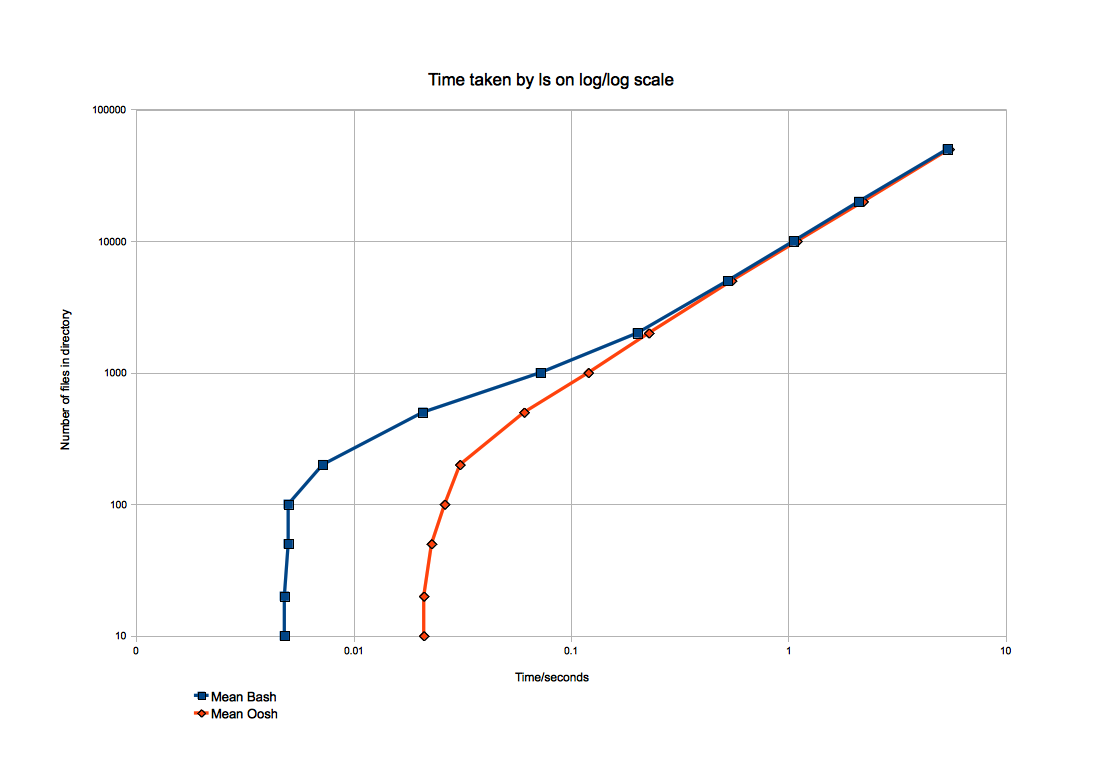
\includegraphics[scale=0.5]{ls_graph.png}
\end{figure}

This graph demonstrates that there is very little performance overhead
when using Oosh for large datasets. At the lower end, Oosh has a
startup time of approximately 0.02 seconds which can be attributed to
the startup time of the Python interpreter. This difference is below
the level of human perception, although pathological cases probably
exist, such as an Oosh script with many short lived processes. A human
being cannot perceive delays of less than 0.1 seconds 
% Card, S K, Moran, T P and Newell, A. The Psychology of
% Humam-Computer Interaction
so this delay is acceptable. Both {\tt ls} and {\tt oosh\_ls} can be
seen to be scaling linearly with respect to the number of files.

Testing {\tt oosh\_ls} scaling allowed me to analyse the costs
introduced by produced by my data structure. If we consider a sample
piece of output from {\tt oosh\_ls} being run on the root directory,
we obtain figure \ref{lsroot}.
% fixme: producing wrong cross-references

\begin{figure}
\label{lsroot}
\caption{Output of {\tt oosh\_ls /} without pretty printing}
\begin{verbatim}
{'Owner': 'root', 'Size': 4096, 'Filename': 'root'}
{'Owner': 'root', 'Size': 4096, 'Filename': 'media'}
{'Owner': 'root', 'Size': 0, 'Filename': '.servers'}
{'Owner': 'root', 'Size': 0, 'Filename': '.ux'}
{'Owner': 'root', 'Size': 3072, 'Filename': 'boot'}
{'Owner': 'wrah2', 'Size': 512, 'Filename': 'apps'}
{'Owner': 'root', 'Size': 12288, 'Filename': 'etc'}
{'Owner': 'root', 'Size': 4540, 'Filename': 'dev'}
{'Owner': 'root', 'Size': 0, 'Filename': 'proc'}
{'Owner': 'root', 'Size': 4096, 'Filename': 'opt'}
{'Owner': 'root', 'Size': 0, 'Filename': 'servers'}
{'Owner': 'root', 'Size': 36864, 'Filename': 'tmp'}
{'Owner': 'root', 'Size': 12288, 'Filename': 'authcon'}
{'Owner': 'root', 'Size': 12288, 'Filename': 'sbin'}
{'Owner': 'root', 'Size': 0, 'Filename': 'sys'}
{'Owner': 'root', 'Size': 12288, 'Filename': 'lib'}
{'Owner': 'root', 'Size': 4096, 'Filename': 'bin'}
{'Owner': 'root', 'Size': 4096, 'Filename': 'usr'}
{'Owner': 'root', 'Size': 4096, 'Filename': 'var'}
{'Owner': 'wrah2', 'Size': 512, 'Filename': 'ux'}
{'Owner': 'root', 'Size': 4096, 'Filename': 'srv'}
{'Owner': 'root', 'Size': 4096, 'Filename': 'mnt'}
{'Owner': 'root', 'Size': 16384, 'Filename': 'lost+found'}
{'Owner': 'root', 'Size': 12288, 'Filename': 'home'}
\end{verbatim}
\end{figure}

As text data this is 1243 bytes, yet {\tt gzip} will compress it to
only 251 bytes. Even allowing for the fact that all ASCII text has
some scope for compression, there is clearly redundancy and inefficiency in the
data format. However this data is typically sent locally, and since
this data is sent via local inter-process communication we have a lot
of bandwidth and can afford the additional overhead of Oosh structured
data. As discussed in section \ref{othermeasures}, CPU consumption is
more of a concern with Oosh so introducing compression would be
unlikely to be a useful optimisation.

\subsection{Latencies introduced by pretty printing}

As discussed in section \ref{prettyimpl}, my pretty printing algorithm
is $O(C \log C + CL)$ in time, where $C$ is the number of columns and
$L$ the number of lines. Under the assumption that a typical workload
will have vastly more lines than columns in the output, I measured
the additional time taken for output to be shown to the user if my
pretty print algorithm is used.

\begin{figure}[h]
\caption{Added latency due to running pretty print algorithm on Oosh
  output}
\centering
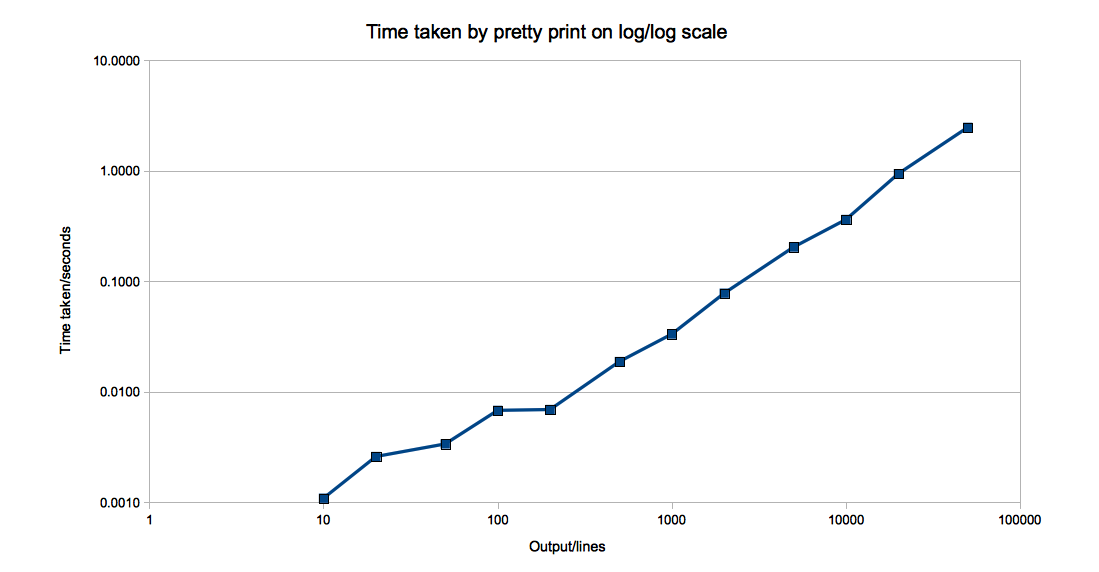
\includegraphics[scale=0.5]{print_graph.png}
\end{figure}

This graph was produced using the same set of directories as in the
previous benchmark, and similarly using {\tt oosh\_ls}. I then
compared time for the command to terminate when with and without
pretty printing.

This graph conceals the fact that the pretty print algorithm requires
the full input before producing any output, whereas the simplistic
Bash-style approach of writing output asynchronously reduces the
perceived latency. The algorithm performs as expected, scaling roughly
linearly as the number of lines increases. Since printing 1000 lines
introduces only 33 milliseconds of delay (on top of the 93
milliseconds required by the rest of the command execution), the
performance of Oosh's pretty print is completely acceptable for small
or medium sized quantities of data.

\subsection{Other measures}
\label{othermeasures}

I also performed a few simpler measures of resource
utilisation. Whilst performing my benchmarks on the most recent build
of Oosh, I used the Linux resource monitor to measure peak system
usage. Memory usage peaked at 43MiB, and CPU usage at 40\%. The memory
consumption is acceptable on a modern systems which tend to have at
least 2GiB of memory. However CPU usage is rather high and since many
experienced shell users often have a number of shells open at once,
this may become a problem.

By contrast, % need some Bash measures here

% what was evaluated?
% what were the results?
%   -- no of processes spawned
%   -- length of equivalent bash shells (can use old commands still!)
%   -- network data comparisons (fixed and variable cost increases measured)
%   -- performance
%     -- wall clock time
%     -- memory and CPU usage (never exceeded 43MiB memory during
%     benchmarks, or 40% CPU)
% testing/debugging
% comparing against requirements

\cleardoublepage
\chapter{Conclusions}

% aims again
% accomplishments -- likes, dislikes, results
% hindsight thoughts -- better approaches
% future prospects

Characterising typical shell usage is difficult. I believe I created a
compelling product. Ultimately very complex shell interactions are often moved
to standalone applications. % contrast Gentoo's build scripts, a distro (Debian?)
                           % moving to C init scripts

The shell is used for quick and dirty tasks, collecting debugging output, simple
file manipulations. Spawning processes ({\tt /etc/init.d/apache start}) and
hardware configuration ({\tt ifconfig}) are also common shell usages which
neither networking convenience or structured data can offer any great
improvement on. Pervasive use of this data structure would offer more
interesting usages, one good example being the {\tt /sys} directory. Tab
completion would be another interesting area to explore, since commands can know
column names (e.g. column name tab completion on oosh\_sort). To be used in
production, Oosh would need to have the remaining shell features added, such as
regular expression support (easy exercise given Python's support). Subshells and
subcommands would be useful to a real user, though not adding anything to the
proof-of-concept design.

% also problems with some data simply not being structured: apt-get upgrade,
% wget, sophisticated interfaces: nano, emacs, irssi, lynx
% line continuations would be nice too

I did not take advantage of any of the optimising flags or profiling
tools within Python, so there is some potential for
improvement. Nonetheless, Oosh performance is not much worse than that
of Bash.

\cleardoublepage

%%%%%%%%%%%%%%%%%%%%%%%%%%%%%%%%%%%%%%%%%%%%%%%%%%%%%%%%%%%%%%%%%%%%%
% the bibliography

\addcontentsline{toc}{chapter}{Bibliography}
\begin{thebibliography}{8} % at most 8 citations

\bibitem{multics}
  Louis Pouzin
  \emph{Multics: The Origin of the Shell}
  http://www.multicians.org/shell.html

\bibitem{bourne}
  Tom Duff
  \emph{Rc -- A Shell for Plan 9 and UNIX systems}
  http://doc.cat-v.org/plan\_9/4th\_edition/papers/rc

\bibitem{fishdesign}
  Axel Liljencrantz
  \emph{Design Document}
  http://fishshell.org/user\_doc/design.html

\bibitem{busybox}
  Denys Vlasenko
  \emph{BusyBox: The Swiss Army Knife of Embedded Linux}
  http://www.busybox.net/about.html

\bibitem{clifu}
  David Winterbottom
  \emph{commandlinefu.com is the place record those command-line gems that
  you return to again and again}
  http://www.commandlinefu.com

\bibitem{bashman}
  Free Software Foundation
  \emph{GNU bash manual}
  http://www.gnu.org/software/bash/manual/

\end{thebibliography}
\cleardoublepage

%%%%%%%%%%%%%%%%%%%%%%%%%%%%%%%%%%%%%%%%%%%%%%%%%%%%%%%%%%%%%%%%%%%%%
% the appendices
\appendix

\chapter{Benchmark data}

\chapter{Project Proposal}
% assumes we are compiling the dissertation using makepdf.sh
% use same formatting as proposal had in header
\parindent 0pt
\parskip 6pt
\include{proposal_include}

\end{document}
